\section{Architectural Design}
Translating the abstract UML models into a functioning codebase requires the selection of an overarching architectural pattern. The SERS application utilizes the Model-View-Controller (MVC) paradigm, heavily augmented by an asynchronous message-brokering layer. The MVC pattern enforces a rigorous separation of concerns. The Model layer encapsulates all business logic, data validation, and database interactions. The View layer is strictly confined to presentation logistics, rendering the user interface and accepting input. The Controller acts as the central orchestrator, receiving HTTP requests from the View, commanding the Model to update its state, and managing the application flow.

However, standard MVC is fundamentally synchronous; a Controller typically blocks the server thread until a task completes. For a reminder system, holding an HTTP connection open for three days until a scheduled event occurs is architecturally catastrophic. Therefore, the technology stack is designed to offload temporal logic. The backend Controller and Model are constructed using Python and the Flask framework. Data is persisted using an SQLite database (capable of scaling to PostgreSQL) mapped via SQLAlchemy. Crucially, the asynchronous layer utilizes Celery as the task queue manager and Redis as the in-memory message broker. When the Flask Controller receives a scheduling request, it pushes the task parameters into the Redis broker and immediately responds to the user. Independent Celery worker processes continuously monitor the Redis broker, executing the tasks only when their specific temporal conditions are met.


\begin{figure}
	\centering
	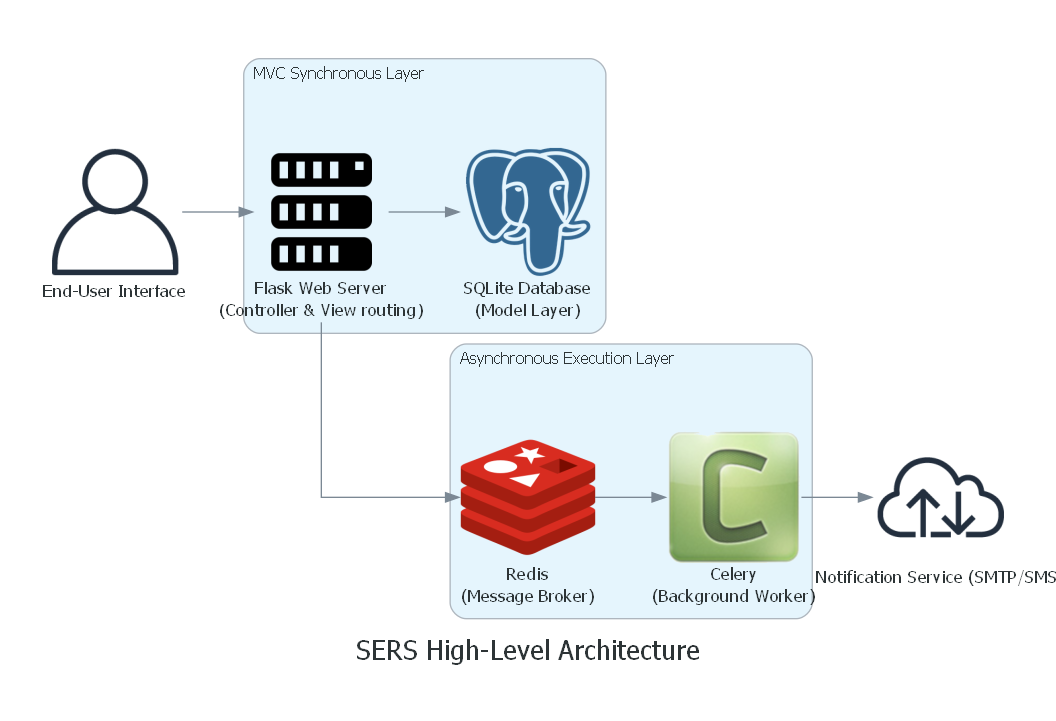
\includegraphics[width=0.8\textwidth]{images/high-level_architecture.png}
	\caption{High-Level Architectural Diagram of the SERS Application}
	\label{fig:architectural-diagram}
\end{figure}
As shown in Figure~\ref{fig:architectural-diagram}, the architecture separates synchronous request handling from asynchronous event execution to keep the system responsive while managing long-delay reminders.

\subsection{Component Roles}
\begin{itemize}
	\item \textbf{User Interface (View Layer):} This component represents the frontend graphical interface where users interact with the system to schedule or manage their events.
	\item \textbf{Flask Web Server (Controller Layer):} This acts as the central orchestrator that receives HTTP requests from the user, validates input logic, and communicates with both the database and the message broker.
	\item \textbf{SQLite Database (Model Layer):} This component persists the application's core data, maintaining the structure and history of all scheduled events and users.
	\item \textbf{Redis (Message Broker):} Functions as a temporary, in-memory queue that holds the task parameters and calculated trigger times for upcoming notifications.
	\item \textbf{Celery (Background Worker):} An independent process that continuously monitors the message broker, executing the notification logic only when the scheduled time arrives.
	\item \textbf{Notification Service:} The external API or SMTP server responsible for actually delivering the reminder message to the end-user.
\end{itemize}

\subsection{Data Flow}
\begin{enumerate}
	\item \textbf{Synchronous Capture:} The user submits a new event via the interface. The Controller receives this data, invokes the Model to save it in the SQLite database, and retrieves a unique Event ID.
	\item \textbf{Asynchronous Offload:} The Controller calculates the exact temporal offset for the reminder. Instead of waiting, it pushes a message payload (containing the Event ID and trigger time) into the Redis Message Broker.
	\item \textbf{Immediate Return:} The Controller immediately returns a success response to the User Interface, freeing up the web server.
	\item \textbf{Deferred Execution:} The Celery Background Worker listens to the Redis queue. When the time constraint is met, Celery pulls the payload and pushes the data outward to the external Notification Service.
\end{enumerate}

\subsection{Architectural Fit} This augmented Model-View-Controller (MVC) pattern is specifically chosen because traditional, strictly synchronous MVC cannot handle long-delayed tasks. By separating the architecture into a synchronous "web layer" and an asynchronous "event-driven layer", the application becomes highly scalable and responsive. The web server is never blocked waiting for a timer to expire, which means the user interface remains fast even if there are thousands of scheduled events waiting in the background. Furthermore, if the notification service experiences an outage, the message broker ensures the event tasks are safely queued and not lost.
\section{Implementation \& Code Quality}
The theoretical architecture is demonstrated in the following Python implementation snippet, which encapsulates the Controller logic and the Celery background worker.

\codefile{python}{code/code.py}

The inspection process focuses on identifying Code Smells—structural indicators of poor design that, while not necessarily preventing the program from functioning, significantly increase technical debt and the probability of future catastrophic failures.

\renewcommand{\arraystretch}{1.3}
\begin{longtable}{|>{\raggedright\arraybackslash}p{0.22\textwidth}|>{\raggedright\arraybackslash}p{0.35\textwidth}|>{\raggedright\arraybackslash}p{0.35\textwidth}|}
	\caption{Identified Code Smells and Refactoring Strategies}\label{tab:identified-code-smells-refactoring} \\
	\hline
	\textbf{Identified Code Smell Category} & \textbf{Technical Description and Observation} & \textbf{Proposed Refactoring Strategy} \\
	\hline
	\endfirsthead

	\hline
	\textbf{Identified Code Smell Category} & \textbf{Technical Description and Observation} & \textbf{Proposed Refactoring Strategy} \\
	\hline
	\endhead

	\hline
	\endfoot

	\hline
	\endlastfoot

	Bloater: Long Method &
	The \texttt{schedule\_new\_event} method handles input validation, database instantiation, complex mathematical time calculations, and asynchronous message brokering simultaneously. It violates the Single Responsibility Principle by attempting to manage too many disparate layers of logic.3 &
	Extract Method: The mathematical calculation of the temporal offset and the actual dispatching to the Celery broker should be abstracted into a private helper function (e.g., \texttt{\_dispatch\_to\_broker()}). This isolates the temporal logic, making the primary method vastly more readable and testable.3 \\
	\hline
	Object-Orientation Abuser: Primitive Obsession &
	Passing discrete primitive variables (\texttt{title}, \texttt{event\_timestamp}, \texttt{target\_email}, \texttt{offset\_minutes}) linearly through multiple architectural layers heavily clutters the method signatures, resulting in Long Parameter Lists and code duplication.49 &
	Introduce Parameter Object: The isolated primitives should be grouped into a single cohesive Data Transfer Object (DTO) or a formalized validation model (such as a Pydantic schema). Passing a single \texttt{EventPayload} object ensures strict type safety across boundaries.3 \\
	\hline
	Concurrency Anti-Pattern: Unsafe Logging &
	Utilizing \texttt{open("system\_delivery\_logs.txt", "a")} directly within the asynchronous worker is highly dangerous. If multiple Celery workers attempt to append to the same text file simultaneously, it will result in file lock collision errors and lost data. &
	Implementation Refactor: Remove raw file I/O operations from background workers. Replace with a thread-safe Python logging module configuration or route logs through a secondary stream processing broker. \\
	\hline
\end{longtable}

 